% MATH 578 FINAL (F16)
% LUKE WUKMER

\documentclass[10pt]{article}

% note: some of these are extremely useful and i don't remember why :o
%\usepackage{savetrees} % disable custom geometry stuff if you do this
\usepackage{titling}    % contol over title & stuff
\usepackage{amsmath, amsthm, amssymb, amsfonts}
\usepackage{amsxtra, amscd, geometry, graphicx}
\usepackage{endnotes}
\usepackage{cancel}
\usepackage{wrapfig}    %inline figs
\usepackage{bm} %allows fancy stuff like bold greek in math mode
\usepackage{alltt}
\usepackage{enumerate} %more/easier control over lists, also see enumitem
%\usepackage[all,cmtip]{xypic}
\usepackage{mathrsfs}
\usepackage{listings} % code with syntax highlighting etc
\usepackage{caption}
\usepackage[raggedright]{sidecap} % side captions
\usepackage{tabu}     % more customizable tables
%\usepackage{subfigure}
%\usepackage{subcaption}
%\usepackage[pdftex]{hyperref}
%\usepackage[dvips,bookmarks,bookmarksopen,backref,colorlinks,linkcolor={blue},citecolor={blue},urlcolor={blue}](hyperref}

\graphicspath{ {./figs/} }

\usepackage{color}


\definecolor{mygreen}{rgb}{0,0.6,0}
\definecolor{mygray}{rgb}{0.5,0.5,0.5}
\definecolor{mymauve}{rgb}{0.58,0,0.82}

\lstset{ %
basicstyle=\footnotesize,        % the size of the fonts that are used for the code
%breakatwhitespace=false,         % sets if automatic breaks should only happen at whitespace
breaklines=false,                 % sets automatic line breaking
captionpos=t,                    % sets the caption-position to bottom
commentstyle=\color{mygray},    % comment styleh
%  deletekeywords={...},            % if you want to delete keywords from the given language
%  escapeinside={\%*}{*)},          % if you want to add LaTeX within your code
%  extendedchars=true,              % lets you use non-ASCII characters; for 8-bits encodings only, does not work with UTF-8
frame=single,                      % adds a frame around the code
%keepspaces=false,                 % keeps spaces in text, useful for keeping indentation of code (possibly needs columns=flexible)
% columns=flexible,
  keywordstyle=\color{blue},       % keyword style
  language=Python,                 % the language of the code
%  otherkeywords={*,...},           % if you want to add more keywords to the set
%  numbers=left,                    % where to put the line-numbers; possible values are (none, left, right)
%  numbersep=5pt,                   % how far the line-numbers are from the code
%numberstyle=\tiny\color{mygray}, % the style that is used for the line-numbers
%  rulecolor=\color{black},         % if not set, the frame-color may be changed on line-breaks within not-black text (e.g. comments (green here))
showspaces=false,                % show spaces everywhere adding particular underscores; it overrides 'showstringspaces'
showstringspaces=false,          % underline spaces within strings only
%  showtabs=false,                  % show tabs within strings adding particular underscores
%  stepnumber=2,                    % the step between two line-numbers. If it's 1, each line will be numbered
  stringstyle=\color{mymauve},     % string literal style
%  tabsize=2,                      % sets default tabsize to 2 spaces
title=\lstname                   % show the filename of files included with \lstinputlisting; also try caption instead of title
}
% change up the fonts (pick one only)
%\usepackage{times}%
%\usepackage{helvet}%
\usepackage{palatino}%
%\usepackage{bookman}%


% These are italic.
% \theoremstyle{definition}

% These are normal (i.e. not italic).
\theoremstyle{definition}

%\newtheorem{prob}{Problem}[section]
\newtheorem{prob}{Problem}
\newtheorem*{prob*}{Problem}
\newtheorem*{soln*}{Solution}
\newtheorem{soln}{Solution}


% New Commands: Common Math Symbols
\providecommand{\R}{\mathbb{R}}%
\providecommand{\N}{\mathbb{N}}%
\providecommand{\Z}{{\mathbb{Z}}}%
\providecommand{\sph}{\mathbb{S}}%
\providecommand{\Q}{\mathbb{Q}}%
\providecommand{\C}{{\mathbb{C}}}%
\providecommand{\F}{\mathbb{F}}%
\providecommand{\quat}{\mathbb{H}}%

% haha, i originally forked this template from one provided by my abstract
% algebra TA (back in 2012 or something). probably don't need most of these,
% huh. 

% New Commands: Operators
%\providecommand{\Gal}{\operatorname{Gal}}%
%\providecommand{\GL}{\operatorname{GL}}%
%\providecommand{\card}{\operatorname{card}}%
%\providecommand{\coker}{\operatorname{coker}}%
%\providecommand{\id}{\operatorname{id}}%
%\providecommand{\im}{\operatorname{im}}%
%\providecommand{\diam}{{\rm diam}}%
%\providecommand{\aut}{\operatorname{Aut}}%
%\providecommand{\inn}{\operatorname{Inn}}%
%\providecommand{\out}{{\rm Out}}%
%\providecommand{\End}{{\rm End}}%
%\providecommand{\rad}{{\rm Rad}}%
\providecommand{\rk}{{\rm rank}}%
%\providecommand{\ord}{{\rm ord}}%
%\providecommand{\comp}{{\text{ $\scriptstyle \circ$ }}}%
\providecommand{\cl}[1]{\overline{#1}}%
\providecommand{\tr}{{\sf trace}}%
\providecommand{\spn}{{\rm span}}%

\renewcommand{\tilde}[1]{\widetilde{#1}}%
%\numberwithin{equation}{section}

% i like the squiggly ones more. add as needed

\renewcommand{\Psi}{\varPsi}

\newcommand*\rfrac[2]{{}^{#1}\!/_{#2}}

% a very fancy dot product \ip{f}{g}
\newcommand\ip[2]{ \left\langle {#1} , {#2} \right\rangle }

% "s.t." for math mode
\providecommand{\st}{\text{ s.t. }}

% \norm{f} and such, super useful
\newcommand{\norm}[1]{\left\lVert#1\right\rVert}

% determinant
%\newcommand{\det}[1]{\textsf{det}\left(#1\right)}

% jacobian
\providecommand{\J}{\textsf{J}}

% this makes the spacing between lines of font a little bigger
%\newcommand{\spacing}[1]{\renewcommand{\baselinestretch}{#1}\large\normalsize}
%\spacing{1.2}

\DeclareMathOperator*{\argmin}{arg\,min}
\DeclareMathOperator*{\argmax}{arg\,max}

\newcommand*\mcol[1]{\overset{\big\uparrow}{\underset{\big\downarrow}{#1}}}

% Makes the margin size a little smaller, i gots stuff to say
\geometry{letterpaper,margin=.8in}

% titling stuff (from package titling)
\posttitle{\par\end{center}}
\setlength{\droptitle}{-.5in}
% END PREAMBLE %%%%%%%%%%%%%%%%%%%%%%%%%
%%%%%%%%%%%%%%%%%%%%%%%%%%%%%%%%%%%%%%%%


\begin{document}

\title{Math 578 Final}
\author{Luke Wukmer}
\date{Fall 2016}
\maketitle \thispagestyle{empty} % remove the page number from the first page

\begin{section}{Implementation}

\begin{subsection}{The V-cycle}
\begin{lstlisting}
def vcycle(l,b,e0, A, I, Lchol):
    
    omega = 2/3
    nu1 = 1

    # base case
    if l == 1:
        e_base = linalg.solve(Lchol.T,linalg.solve(Lchol,b))
        return e_base
    else:
        a = A[-(l-1)]
        i = I[-(l-1)]
        e = smooth(a, omega, nu1, b, e0)

        # compute and restrict error
        res = i.T @ (b - a@e)

        # correct error
        e = e + i @ vcycle(l-1,res, np.zeros_like(res), A,I,Lchol)
         
        # smooth nu1 times on a x = b with initial guess e
        e = smooth(a,omega,nu1,b,e)

    return e
\end{lstlisting}
\end{subsection}
\begin{subsection}{Smoothing function}
Here is the smoothing function. As described in the docstring, this function was first tested for accuracy by applying it to a $4\times4$ diagonally dominant system. This system was suggested by the Wikipedia page for Jacobi iteration.
\begin{lstlisting}
def smooth(A, omega, nu, b, x0, tol=None):
    """
    smoothing function via ω-weighted Jacobi iteration
    this is also a standard iterative method on a
    diagonally dominant system



    AA = np.array([[10., -1., 2., 0.],
                   [-1., 11., -1., 3.],
                   [2., -1., 10., -1.],
                   [0.0, 3., -1., 8.]])

    bb = np.array([6., 25., -11., 15.])
    x00 = np.zeros_like(bb)
    ans = smooth(AA,1., 50, bb, x00)

    converges after 24 iterations
    
    if omega is changed to 2/3 in the above, converges in 35 iterations
    """
    if x0.ndim == 1:
        x0 = np.expand_dims(x0,-1)
    if b.ndim == 1:
        b = np.expand_dims(b,-1)
    
    x = x0.copy()
    D = np.diag(A) # diagonal of system (as a Nx1 vector)
    # must be same shape as b or will broadcast to a matrix under division
    D = D.reshape(x.shape)

    W = np.tril(A, k=-1) + np.triu(A,k=1) #deleted diagonal

    for i in range(nu):
        x = (1-omega)*x + ((omega*(b- (W@x))) / D)
        if tol is not None and np.allclose(b,A@x, 1e-12):
            break
    else:
        if tol is not None:
            print("Warning, did not converge within tolerance", tol)

    return x
    \end{lstlisting}
\end{subsection}
\end{section}
\begin{section}{Results}
\begin{verbatim}
In [5]: run mgcg.py
____________________________________________________________
M= 11 L= 6
method: <function interpolation_matrix at 0x7fe7c1569d08>
65 iterations
time elapsed= 7.588343381881714
____________________________________________________________
____________________________________________________________
M= 11 L= 6
method: <function interpolation_matrix_2 at 0x7fe7c1569d90> 
41 iterations
time elapsed= 4.9514479637146
____________________________________________________________
____________________________________________________________
M= 11 L= 6
method: None
512 iterations
time elapsed= 3.9358863830566406
____________________________________________________________
____________________________________________________________
M= 12 L= 7
method: <function interpolation_matrix at 0x7fe7c1569d08>
99 iterations
time elapsed= 45.84742569923401
____________________________________________________________
____________________________________________________________
M= 12 L= 7
method: <function interpolation_matrix_2 at 0x7fe7c1569d90>
61 iterations
time elapsed= 28.84040141105652
____________________________________________________________
____________________________________________________________
M= 12 L= 7
method: None
1024 iterations
time elapsed= 29.221490144729614
____________________________________________________________
____________________________________________________________
M= 13 L= 8
method: <function interpolation_matrix at 0x7fe7c1569d08>
58 iterations
time elapsed= 256.6284234523773
____________________________________________________________
____________________________________________________________
M= 13 L= 8
method: <function interpolation_matrix_2 at 0x7fe7c1569d90>
87 iterations
time elapsed= 154.2831733226776
____________________________________________________________
____________________________________________________________
M= 13 L= 8
method: None
2048 iterations
time elapsed= 230.1282079219818
____________________________________________________________
\end{verbatim}
\end{section}
\begin{section}{The Bonus Question Answered}
If MGCG is performed on the system-in-question $A$ using the interpolation method known as "scenario \#2", the optimal choice of level-depth $L$ is \begin{huge}\textbf{exactly 3}\end{huge} for any size $M\ge3$. That is, the "standard" interpolation method (2) is used to interpolate between $A_L \rightarrow A_{L-1}$ and $A_{L-2}\rightarrow A_{L-3} = A_{1}$, and the "special" interpolation method introduced in scenario \#2 is performed once in between. There are two reasons why, and they are clearly seen from a visual depiction of the multigrid systems of A using scenario \#2.



The following figure was generated with the code \texttt{bonus\_demo.py}. Here we see the four finest systems in the multigrid when $M=7, L=6$, although this result is obviously true for any choice of $M$.
\begin{figure}[p]
\begin{center}
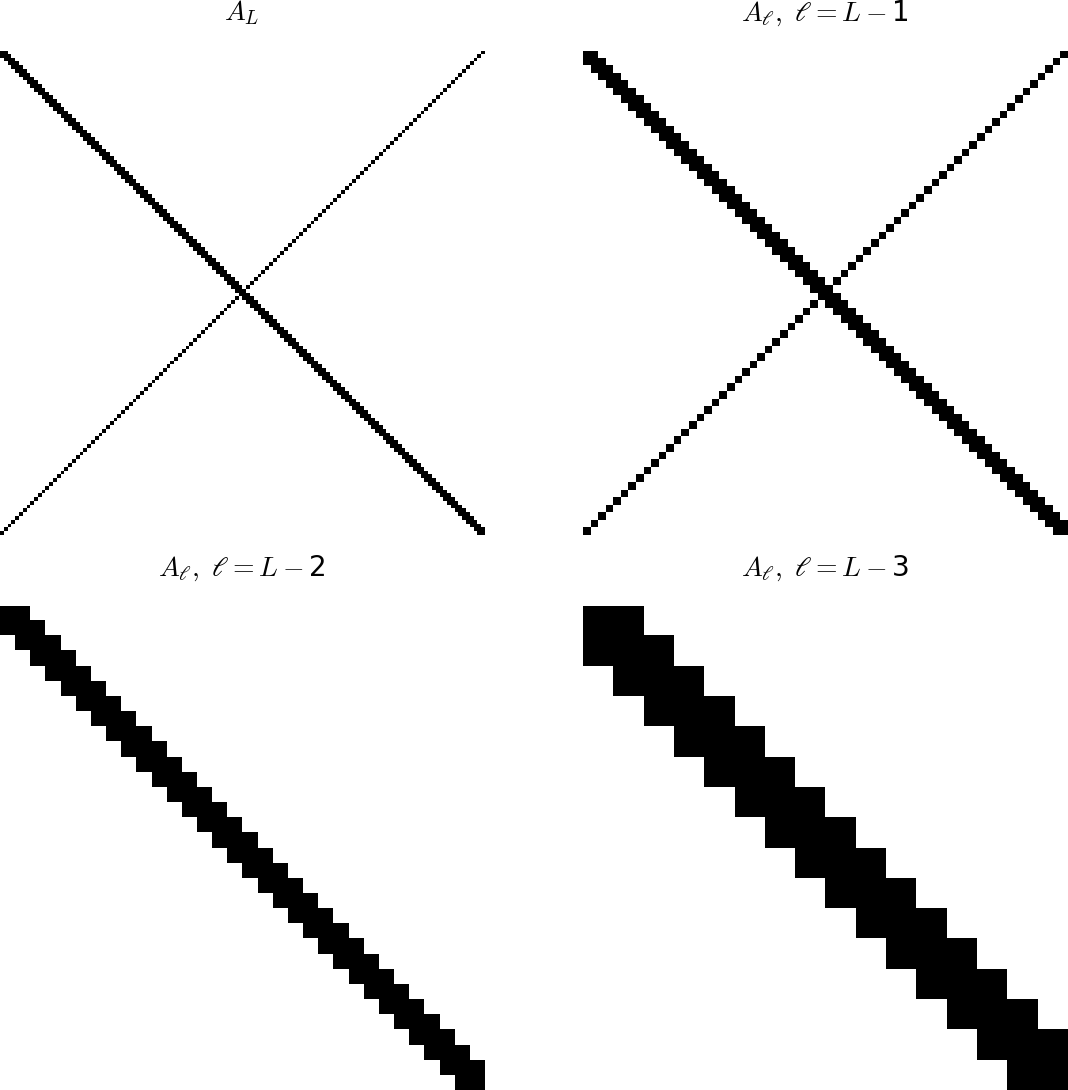
\includegraphics[width=0.8\linewidth]{scenario2_spy.png}
\end{center}
\end{figure}

The result is clear: applying the modified interpolation step between levels $A_{L-1}$ and $A_{L-2}$ converts the system from its original structure (with an antidiagonal) to a tridiagonal matrix, and all further interpolations preserve tridiagonality. Recalling that our goal in the V-cycle is to restrict the size of the system until we arrive at a system that is reasonable to solve directly, it makes sense that we should immediately solve such a system. There will be no additional benefit from successive restriction of the system once it is tridiagonal.

\lstinputlisting{bonus_demo.py}

Of course, since performing the downscaling of the system A isn't computationally "free", we can directly see the superiority of choosing \textit{exactly} 3 levels. The following shows a session in \texttt{ipython}, where we perform the entire MGCG procedure on our system when $M=11$, iterating on the number of levels $L=1,2,\dots,9$. The average runtime over 3 runs is displayed for each L value. 
\begin{verbatim}
In [1]: from mgcg import * 
In [2]: M = 11
In [3]: A = make_system(M)
In [4]: b = np.ones((2**M, 1))/2**(11/2)
In [5]: for L in range(1,10):
  ....:    %timeit mgcg(A,b,L,interpolation_matrix_2)
  ....:     
1 loop, best of 3: 2.65 s per loop
1 loop, best of 3: 1.86 s per loop
1 loop, best of 3: 1.48 s per loop	<-------------------------------
1 loop, best of 3: 2.79 s per loop
1 loop, best of 3: 3.96 s per loop
1 loop, best of 3: 4.99 s per loop
1 loop, best of 3: 6.84 s per loop
1 loop, best of 3: 7.58 s per loop
1 loop, best of 3: 7.9 s per loop
\end{verbatim}

These times are shown in the graph below:
\begin{figure}[p]
\begin{center}
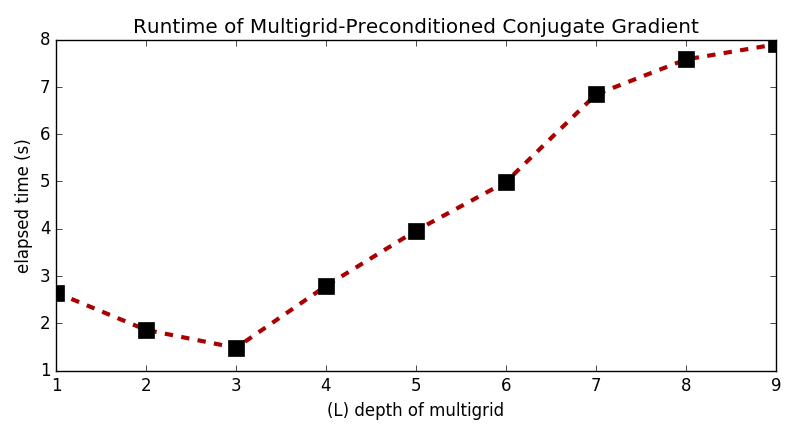
\includegraphics[width=0.8\linewidth]{runtimes.png}
\end{center}
\end{figure}
\end{section}
\end{document}

